
\documentclass[tikz, border=10pt]{standalone}
\usepackage{tikz}
\usepackage{graphicx}
\usepackage{amsmath}
\usetikzlibrary{positioning, shadows, calc, shapes}

\newcommand{\bigcdot}{\cdot} % Fallback

\begin{document}
\section{DeepONet Architecture}
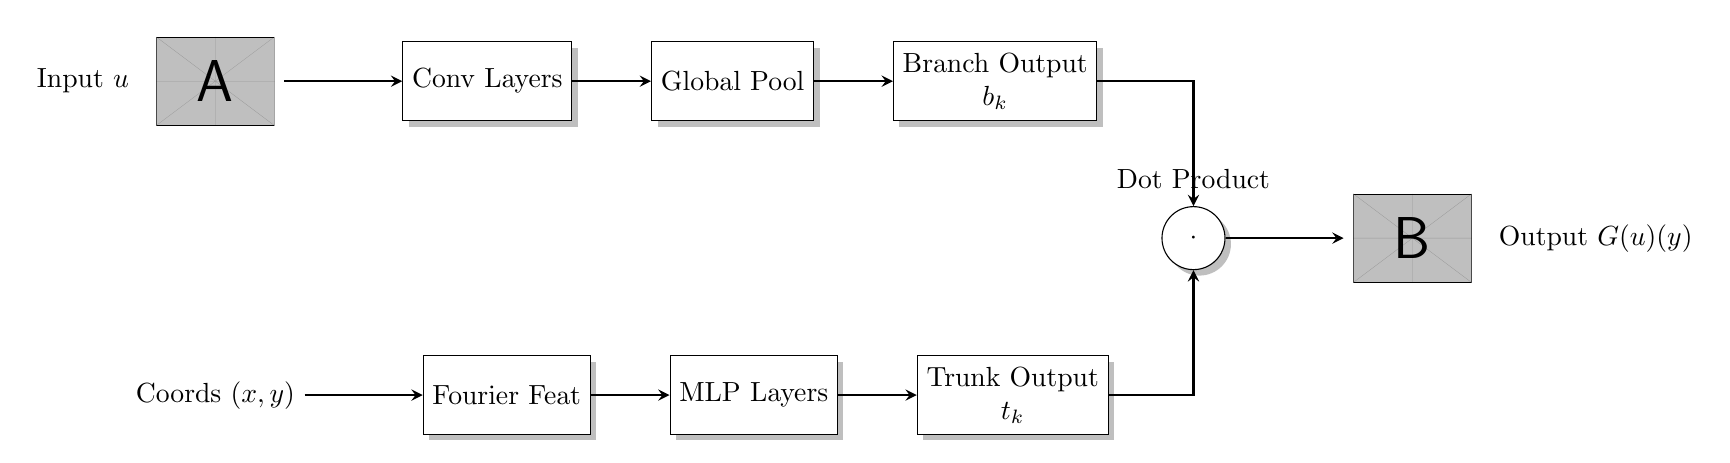
\begin{tikzpicture}[
    node distance=1.5cm,
    block/.style={draw, rectangle, minimum height=1.0cm, minimum width=2.0cm, align=center, fill=white, drop shadow},
    op/.style={draw, circle, minimum size=0.8cm, fill=white, drop shadow},
    arrow/.style={->, >=stealth, thick}
]
    % Branch Net (Top)
    \node (input) {\includegraphics[width=1.5cm]{example-image-a}};
    \node[left=0.1cm of input] {Input $u$};
    
    \node[block, right=1.5cm of input] (branch1) {Conv Layers};
    \node[block, right=1.0cm of branch1] (branch2) {Global Pool};
    \node[block, right=1.0cm of branch2] (branch_out) {Branch Output\\$b_k$};

    % Trunk Net (Bottom)
    \node[below=3.0cm of input] (coords) {Coords $(x,y)$};
    
    \node[block, right=1.5cm of coords] (trunk1) {Fourier Feat};
    \node[block, right=1.0cm of trunk1] (trunk2) {MLP Layers};
    \node[block, right=1.0cm of trunk2] (trunk_out) {Trunk Output\\$t_k$};
    
    % Combine
    \node[op, at={($(branch_out)!0.5!(trunk_out)$)}, right=2.0cm] (dot) {$\bigcdot$};
    \node[above=0.1cm of dot] {Dot Product};

    % Output
    \node[right=1.5cm of dot] (output) {\includegraphics[width=1.5cm]{example-image-b}};
    \node[right=0.1cm of output] {Output $G(u)(y)$};

    % Connections Branch
    \draw[arrow] (input) -- (branch1);
    \draw[arrow] (branch1) -- (branch2);
    \draw[arrow] (branch2) -- (branch_out);
    \draw[arrow] (branch_out) -| (dot);

    % Connections Trunk
    \draw[arrow] (coords) -- (trunk1);
    \draw[arrow] (trunk1) -- (trunk2);
    \draw[arrow] (trunk2) -- (trunk_out);
    \draw[arrow] (trunk_out) -| (dot);

    % Connection Out
    \draw[arrow] (dot) -- (output);

\end{tikzpicture}
\end{document}
